\subsection*{1. Executar os diferentes servidores em uma máquina diferente da
máquina cliente.}
\addcontentsline{toc}{section}{1. Executar os servidores}

Os servidores foram executados em duas máquinas Windows conectadas via Ethernet. O servidor em C foi executado em um subsistema Linux do windows (WSL). Podemos notar pelas figuras abaixo que o desempenho do código utilizando NIO foi muito superior aos outros dois servidores. Por questões de compatibilidade com a IDE e problemas com o uso de pacotes, as classes em java foram renomeadas, mas são, à parte disso, as mesmas do enunciado.

\vspace{2em}
\begin{minipage}{\textwidth}
    \hspace{-1em}
    \centering
    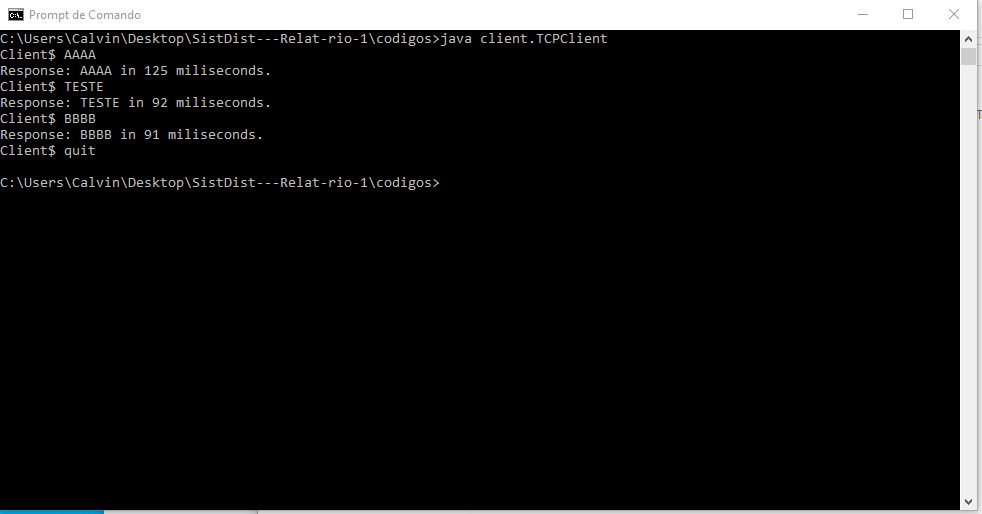
\includegraphics[trim= 0 200 250 0, clip, scale=.4] {prints/terminal-cilente-threaded.JPG}
    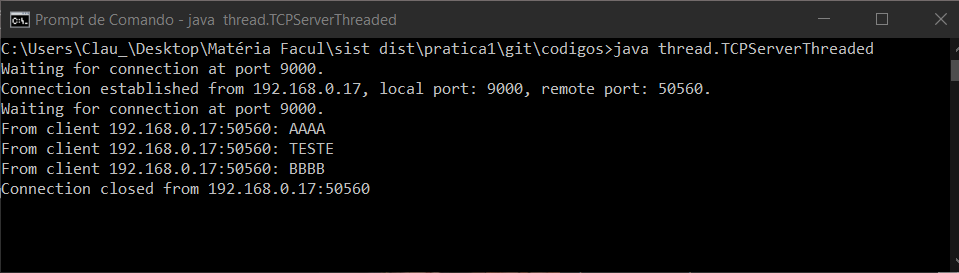
\includegraphics[scale=.4]{prints/terminal-server-threaded.PNG}
    \captionof{figure}{Execução do servidor baseado em threads}
    \label{threadspng}
    \hspace{1em}
\end{minipage}
\vspace{0.5em}

\vspace{2em}
\begin{minipage}{\textwidth}
    \hspace{-1em}
    \centering
    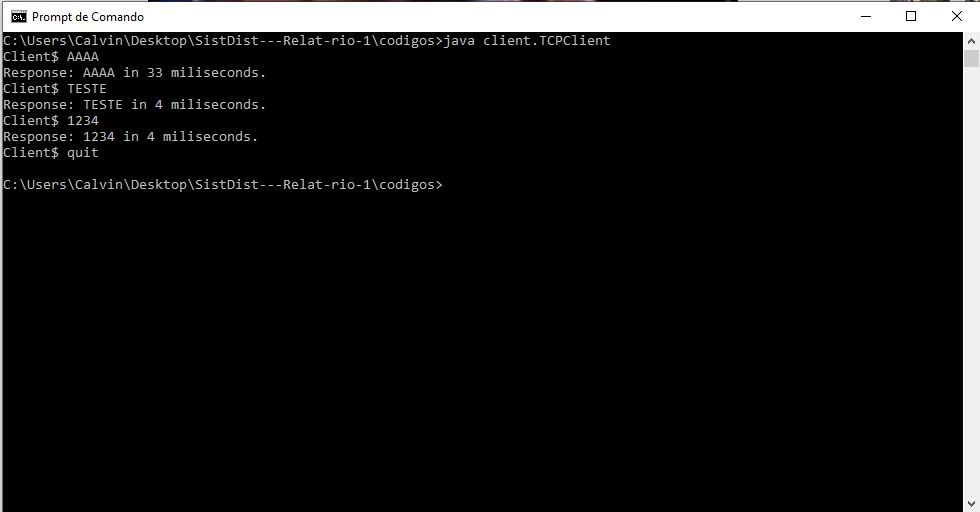
\includegraphics[trim= 0 200 250 0, clip, scale=.4] {prints/terminal-cilente-nio.JPG}
    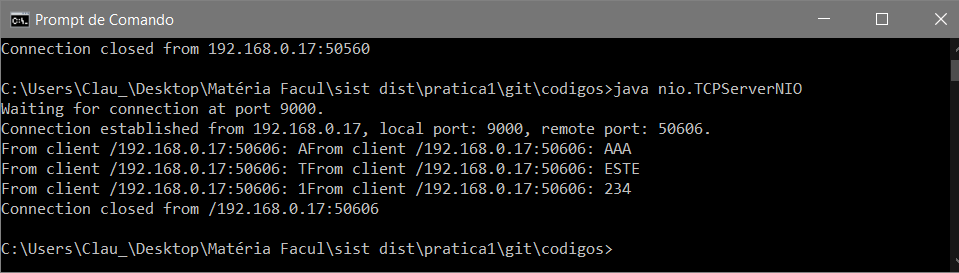
\includegraphics[scale=.4]{prints/terminal-server-nio.PNG}
    \captionof{figure}{Execução do servidor baseado em NIO}
    \label{threadspng}
    \hspace{1em}
\end{minipage}
\vspace{0.5em}

\vspace{2em}
\begin{minipage}{\textwidth}
    \hspace{-1em}
    \centering
    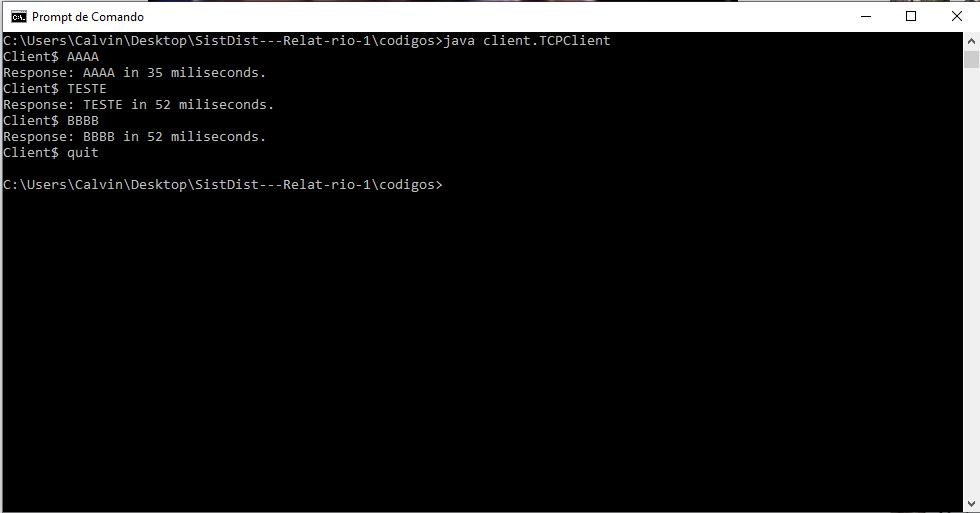
\includegraphics[trim= 0 200 250 0, clip, scale=.4] {prints/terminal-cilente-fork.JPG}
    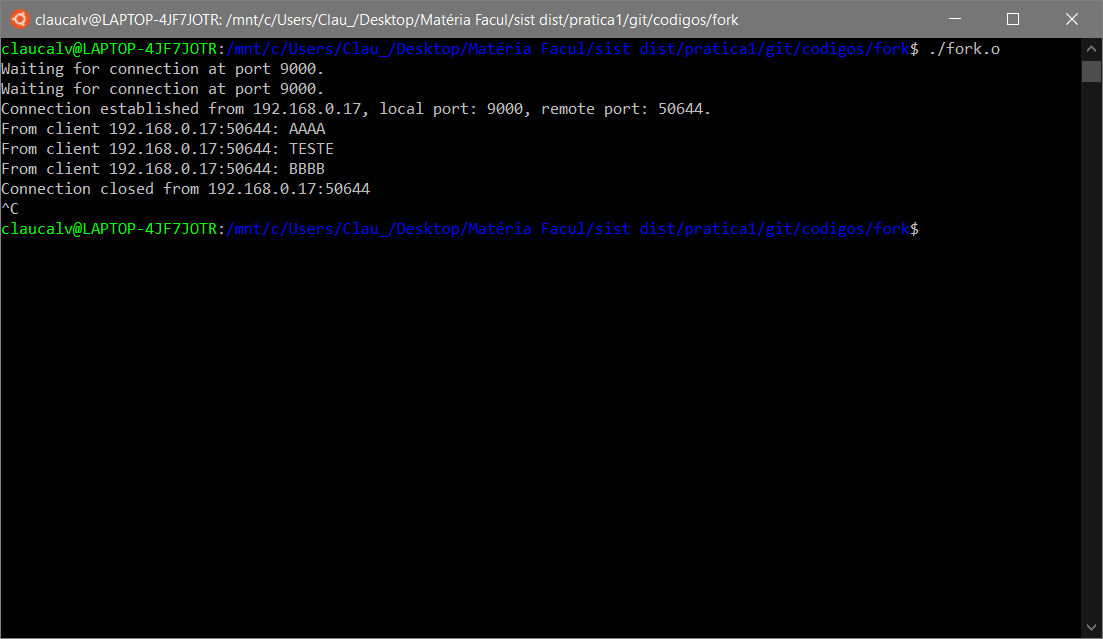
\includegraphics[trim= 0 200 0 0, clip, scale=.4] {prints/terminal-server-fork.PNG}
    \captionof{figure}{Execução do servidor baseado em fork}
    \label{threadspng}
    \hspace{1em}
\end{minipage}
\vspace{0.5em}

\pagebreak

\subsubsection{1.1 - Usar o Visual VM para avaliar o comportamento dos programas em Java, incluindo o desempenho.}
\addcontentsline{toc}{subsection}{1.1 Usar VisualVM}

Além da resposta mais rápida, percebe-se que o servidor NIO não possui o custo das threads extras que o threaded possui.

\vspace{2em}
\begin{minipage}{\textwidth}
    \hspace{-1em}
    \centering
    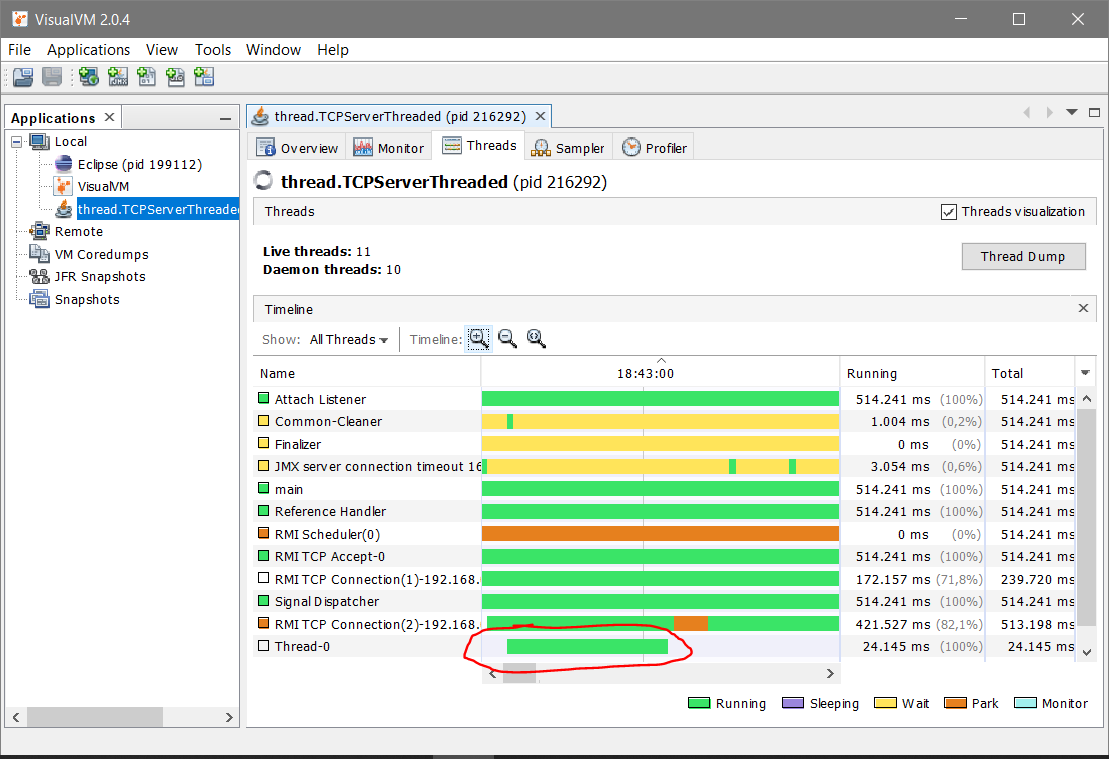
\includegraphics[scale=.4]{prints/visualvm-threaded.PNG}
    \captionof{figure}{Threads do servidor baseado em threads}
    \label{threadspng}
    \hspace{1em}
\end{minipage}
\vspace{0.5em}

\vspace{2em}
\begin{minipage}{\textwidth}
    \hspace{-1em}
    \centering
    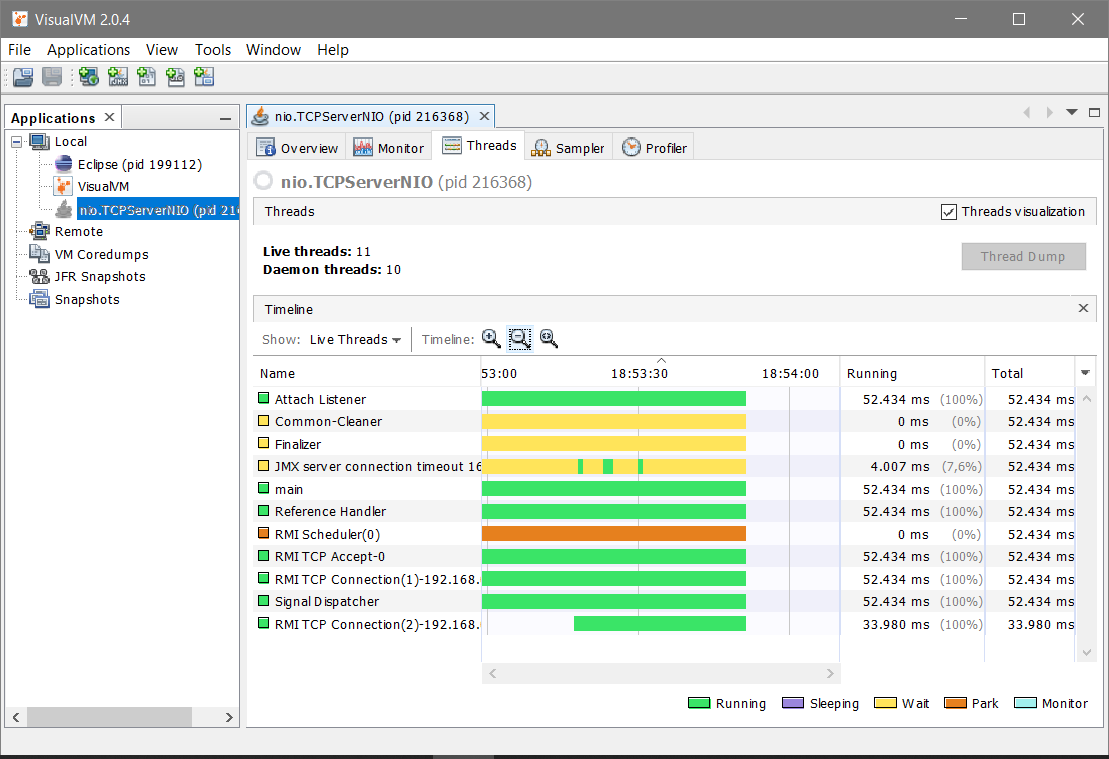
\includegraphics[scale=.4]{prints/visualvm-nio.PNG}
    \captionof{figure}{Threads do servidor baseado em NIO}
    \label{threadspng}
    \hspace{1em}
\end{minipage}
\vspace{0.5em}

\pagebreak

\subsubsection{1.2 - Fazer a captura dos pacotes usando Wireshark e discutir o protocolo de aplicação usado.}
\addcontentsline{toc}{subsection}{1.2 Usar Wireshark}

Podemos ver todos os sinais de um protocolo TCP, a começar pelo handshake de 3 vias, os pacotes de confirmação entre os pacotes de mensagem, e a finalização bidirecional da comunicação.

\vspace{2em}
\begin{minipage}{\textwidth}
    \hspace{-1em}
    \centering
    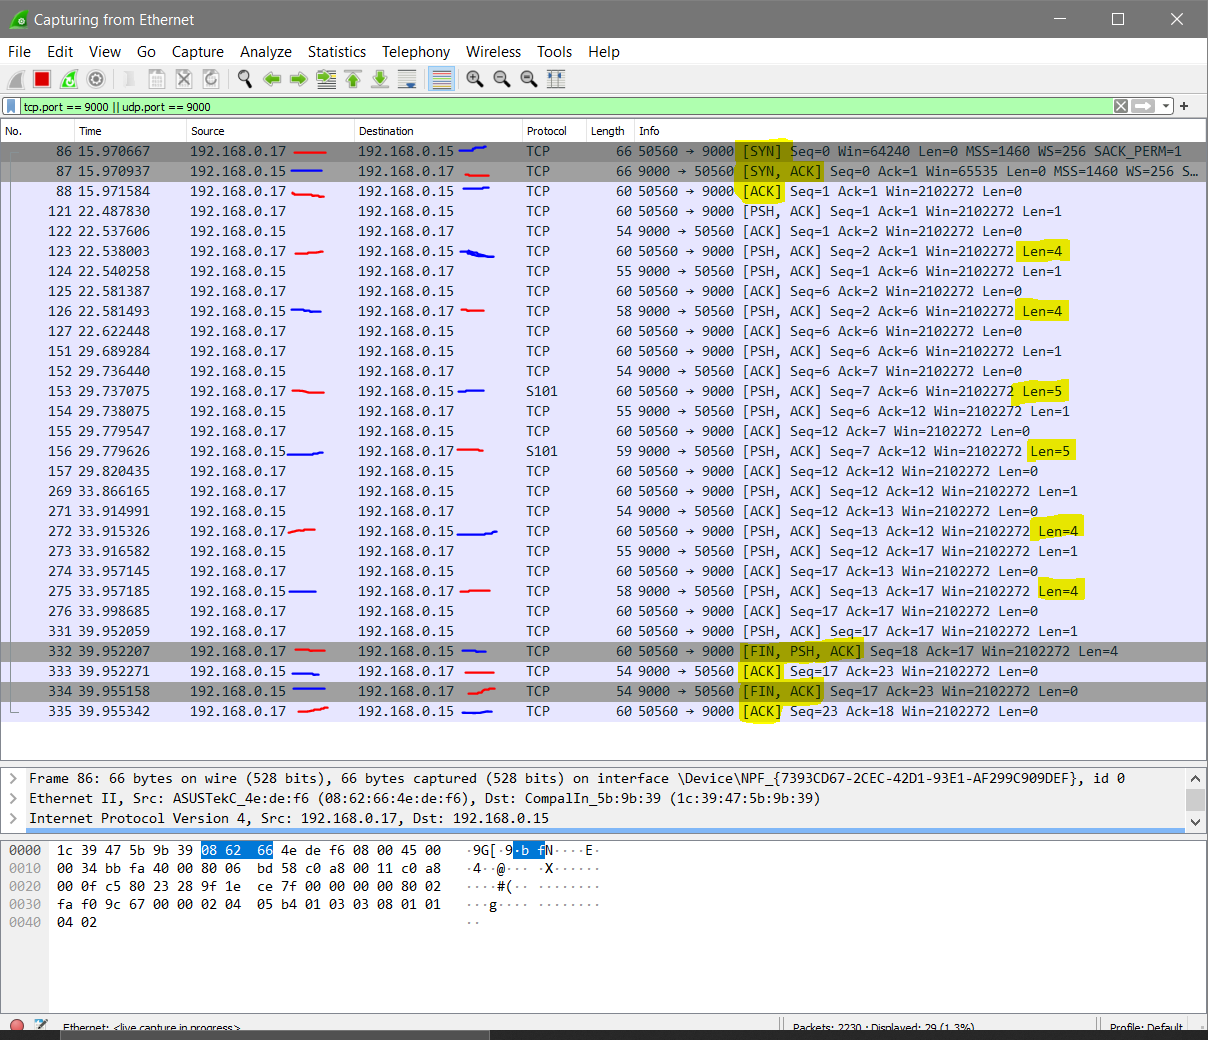
\includegraphics[scale=.3]{prints/wireshark-threaded.PNG}
    \captionof{figure}{Captura de pacotes do servidor baseado em threads}
    \label{threadspng}
    \hspace{1em}
\end{minipage}
\vspace{0.5em}

\vspace{2em}
\begin{minipage}{\textwidth}
    \hspace{-1em}
    \centering
    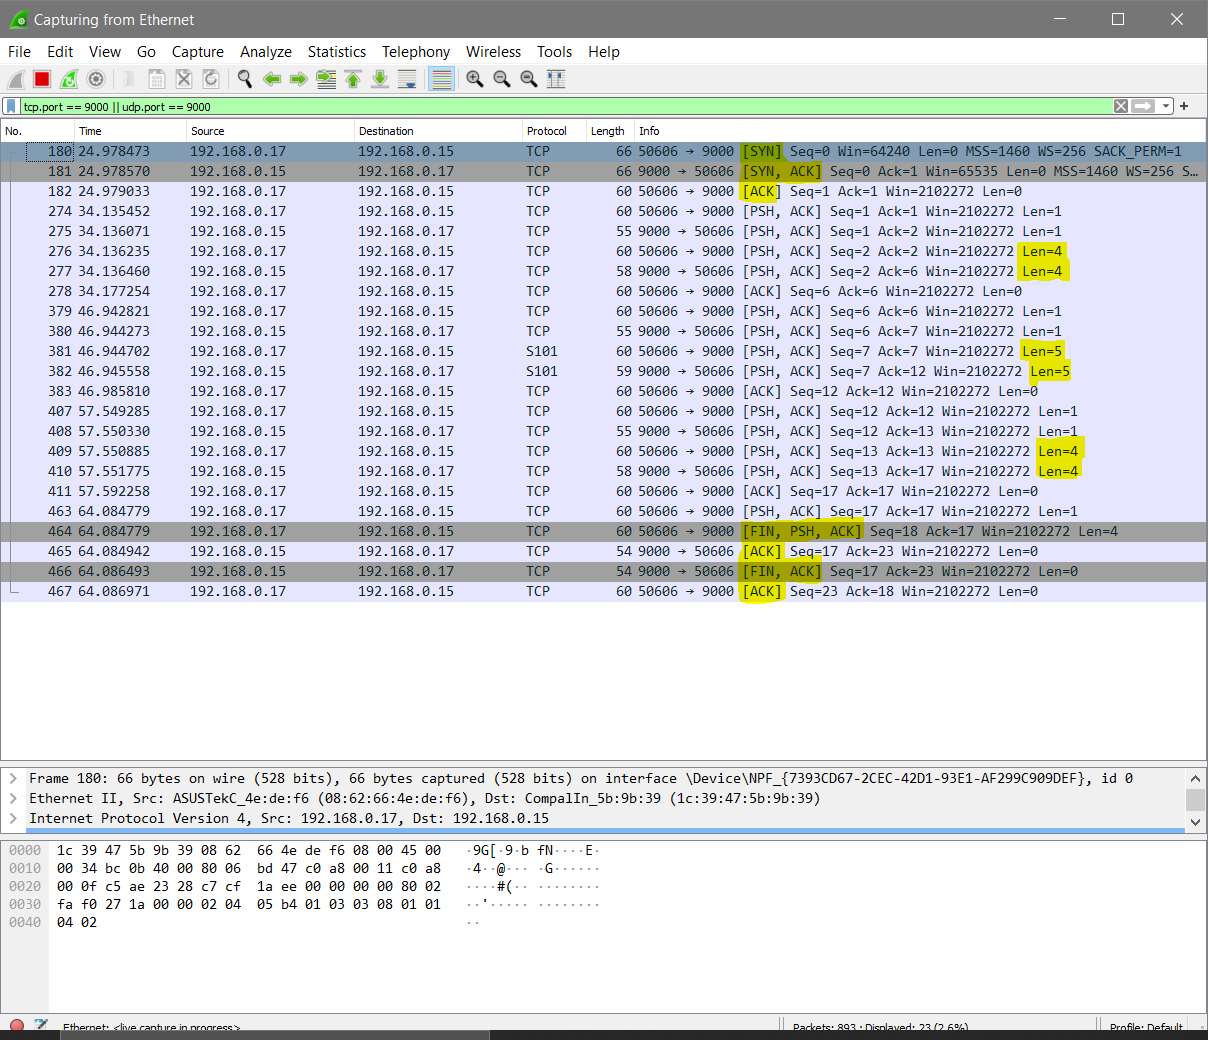
\includegraphics[scale=.3]{prints/wireshark-nio.PNG}
    \captionof{figure}{Captura de pacotes do servidor baseado em NIO}
    \label{threadspng}
    \hspace{1em}
\end{minipage}
\vspace{0.5em}

\vspace{2em}
\begin{minipage}{\textwidth}
    \hspace{-1em}
    \centering
    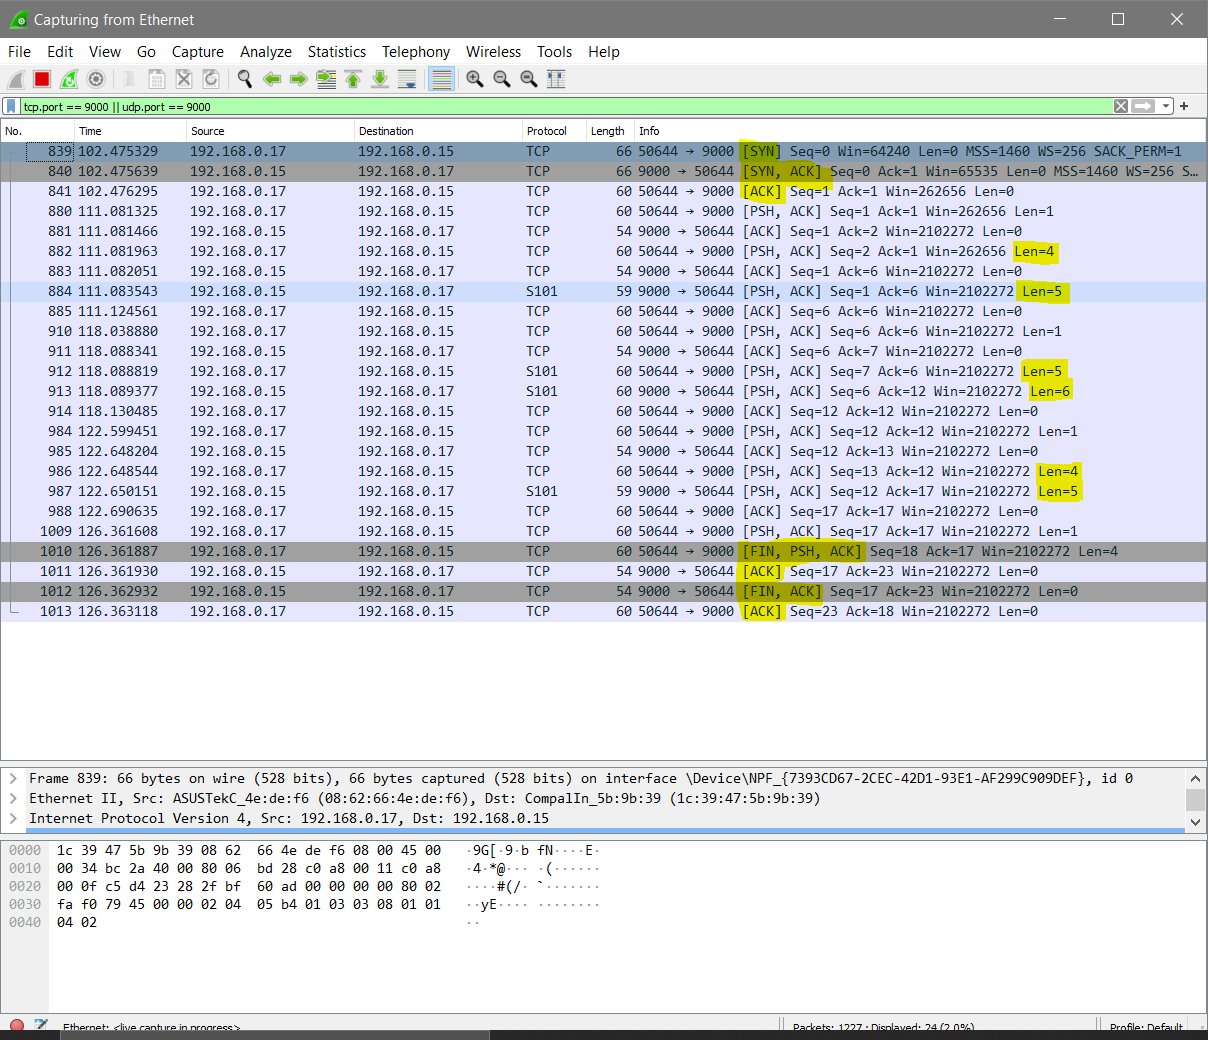
\includegraphics[scale=.3]{prints/wireshark-fork.PNG}
    \captionof{figure}{Captura de pacotes do servidor baseado em fork}
    \label{threadspng}
    \hspace{1em}
\end{minipage}
\vspace{0.5em}

\pagebreak

\subsection*{2. Modificar o servidor Java multi-threaded para usar pool de threads.}
\addcontentsline{toc}{section}{2. Adicionar o pool de threads}

A estrutura base foi adaptada do \hyperlink{http://tutorials.jenkov.com/java-concurrency/thread-pools.html}{tutorial sugerido pelo professor}
, e as principais implementações, na outra figura abaixo, retiradas do código original TCPServerThreaded.

\vspace{-0.5em}
\begin{minipage}{\textwidth}
  \hspace{-1em}
  \centering
  \lstinputlisting[language=Java, linerange={18-37,60-99}] {codigos/threadpool/TCPServerThreadPool.java}
  \captionof{figure}{Estrutura do servidor baseado em threadpool}
  \label{prog1}
  \hspace{1em}
\end{minipage}
\vspace{0.5em}

\vspace{-0.5em}
\begin{minipage}{\textwidth}
  \hspace{-1em}
  \centering
  \lstinputlisting[language=Java, linerange={37-60,100-999}] {codigos/threadpool/TCPServerThreadPool.java}
  \captionof{figure}{Implementação dos métodos TCPThread.work() e main()}
  \label{prog1}
  \hspace{1em}
\end{minipage}
\vspace{0.5em}

\vspace{2em}
\begin{minipage}{\textwidth}
    \hspace{-1em}
    \centering
    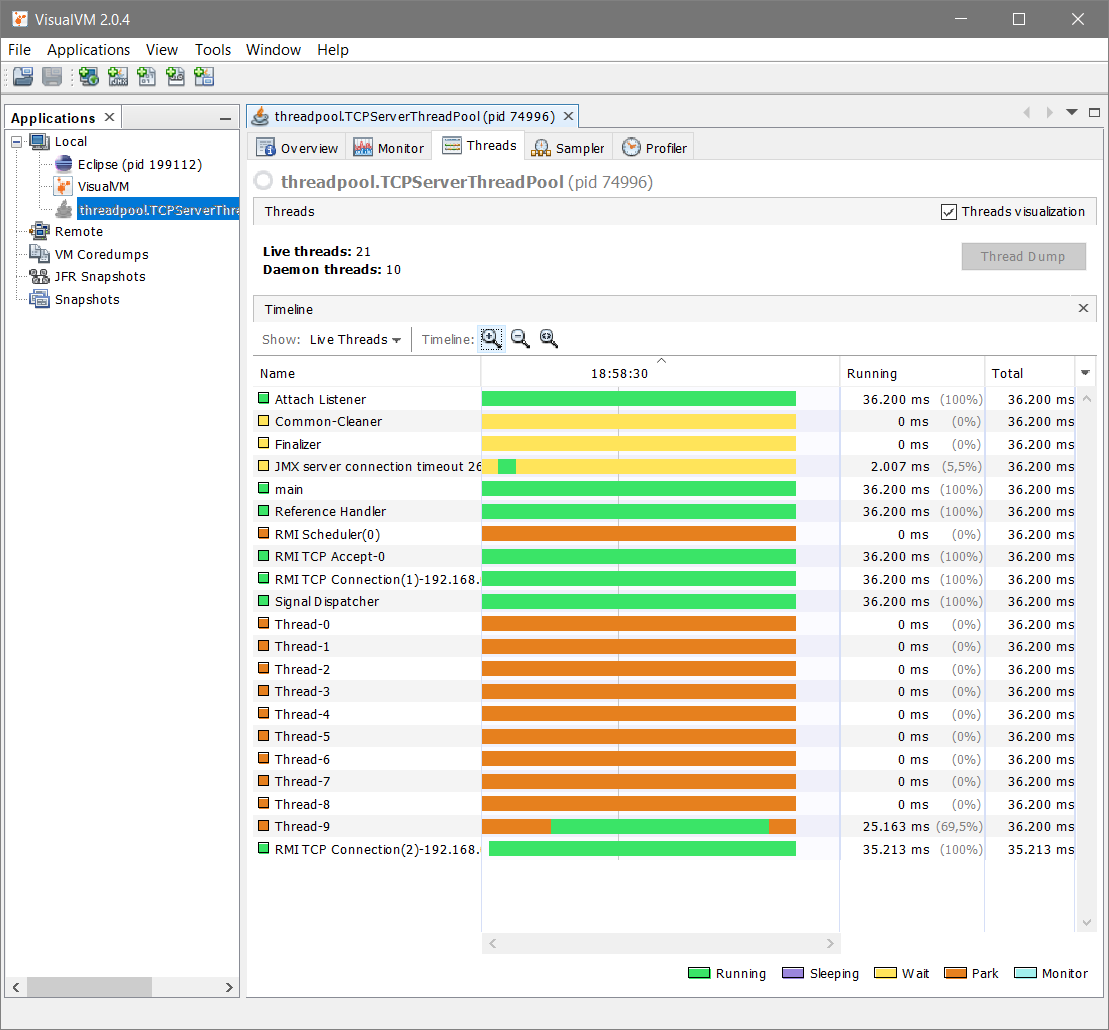
\includegraphics[scale=.4]{prints/visualvm-threadpool.PNG}
    \captionof{figure}{Threads do servidor baseado em threadpool}
    \label{threadspng}
    \hspace{1em}
\end{minipage}
\vspace{0.5em}

\vspace{2em}
\begin{minipage}{\textwidth}
    \hspace{-1em}
    \centering
    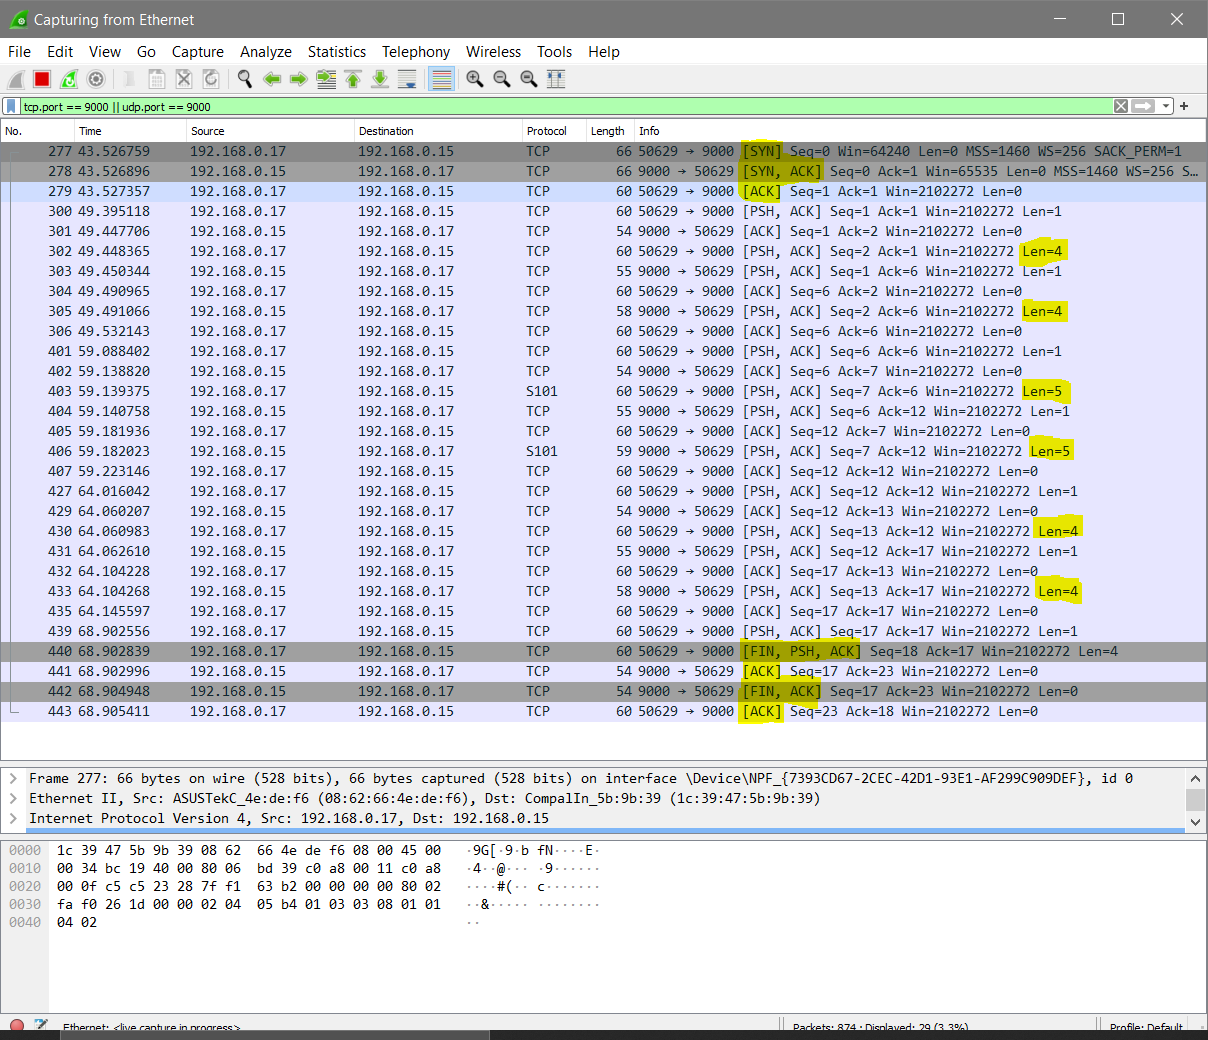
\includegraphics[scale=.3]{prints/wireshark-threadpool.PNG}
    \captionof{figure}{Captura de pacotes do servidor baseado em threadpool}
    \label{threadspng}
    \hspace{1em}
\end{minipage}
\vspace{0.5em}